\newcommand{\matlab}{MATLAB\textsuperscript{\textregistered}}
\chapter{What is \pharmml?}
\label{chap:pharmml-what}

\section{The Problem}

%\begin{figure}[h]
%{
%\centering
\begin{wrapfigure}{r}{0.45\linewidth}
  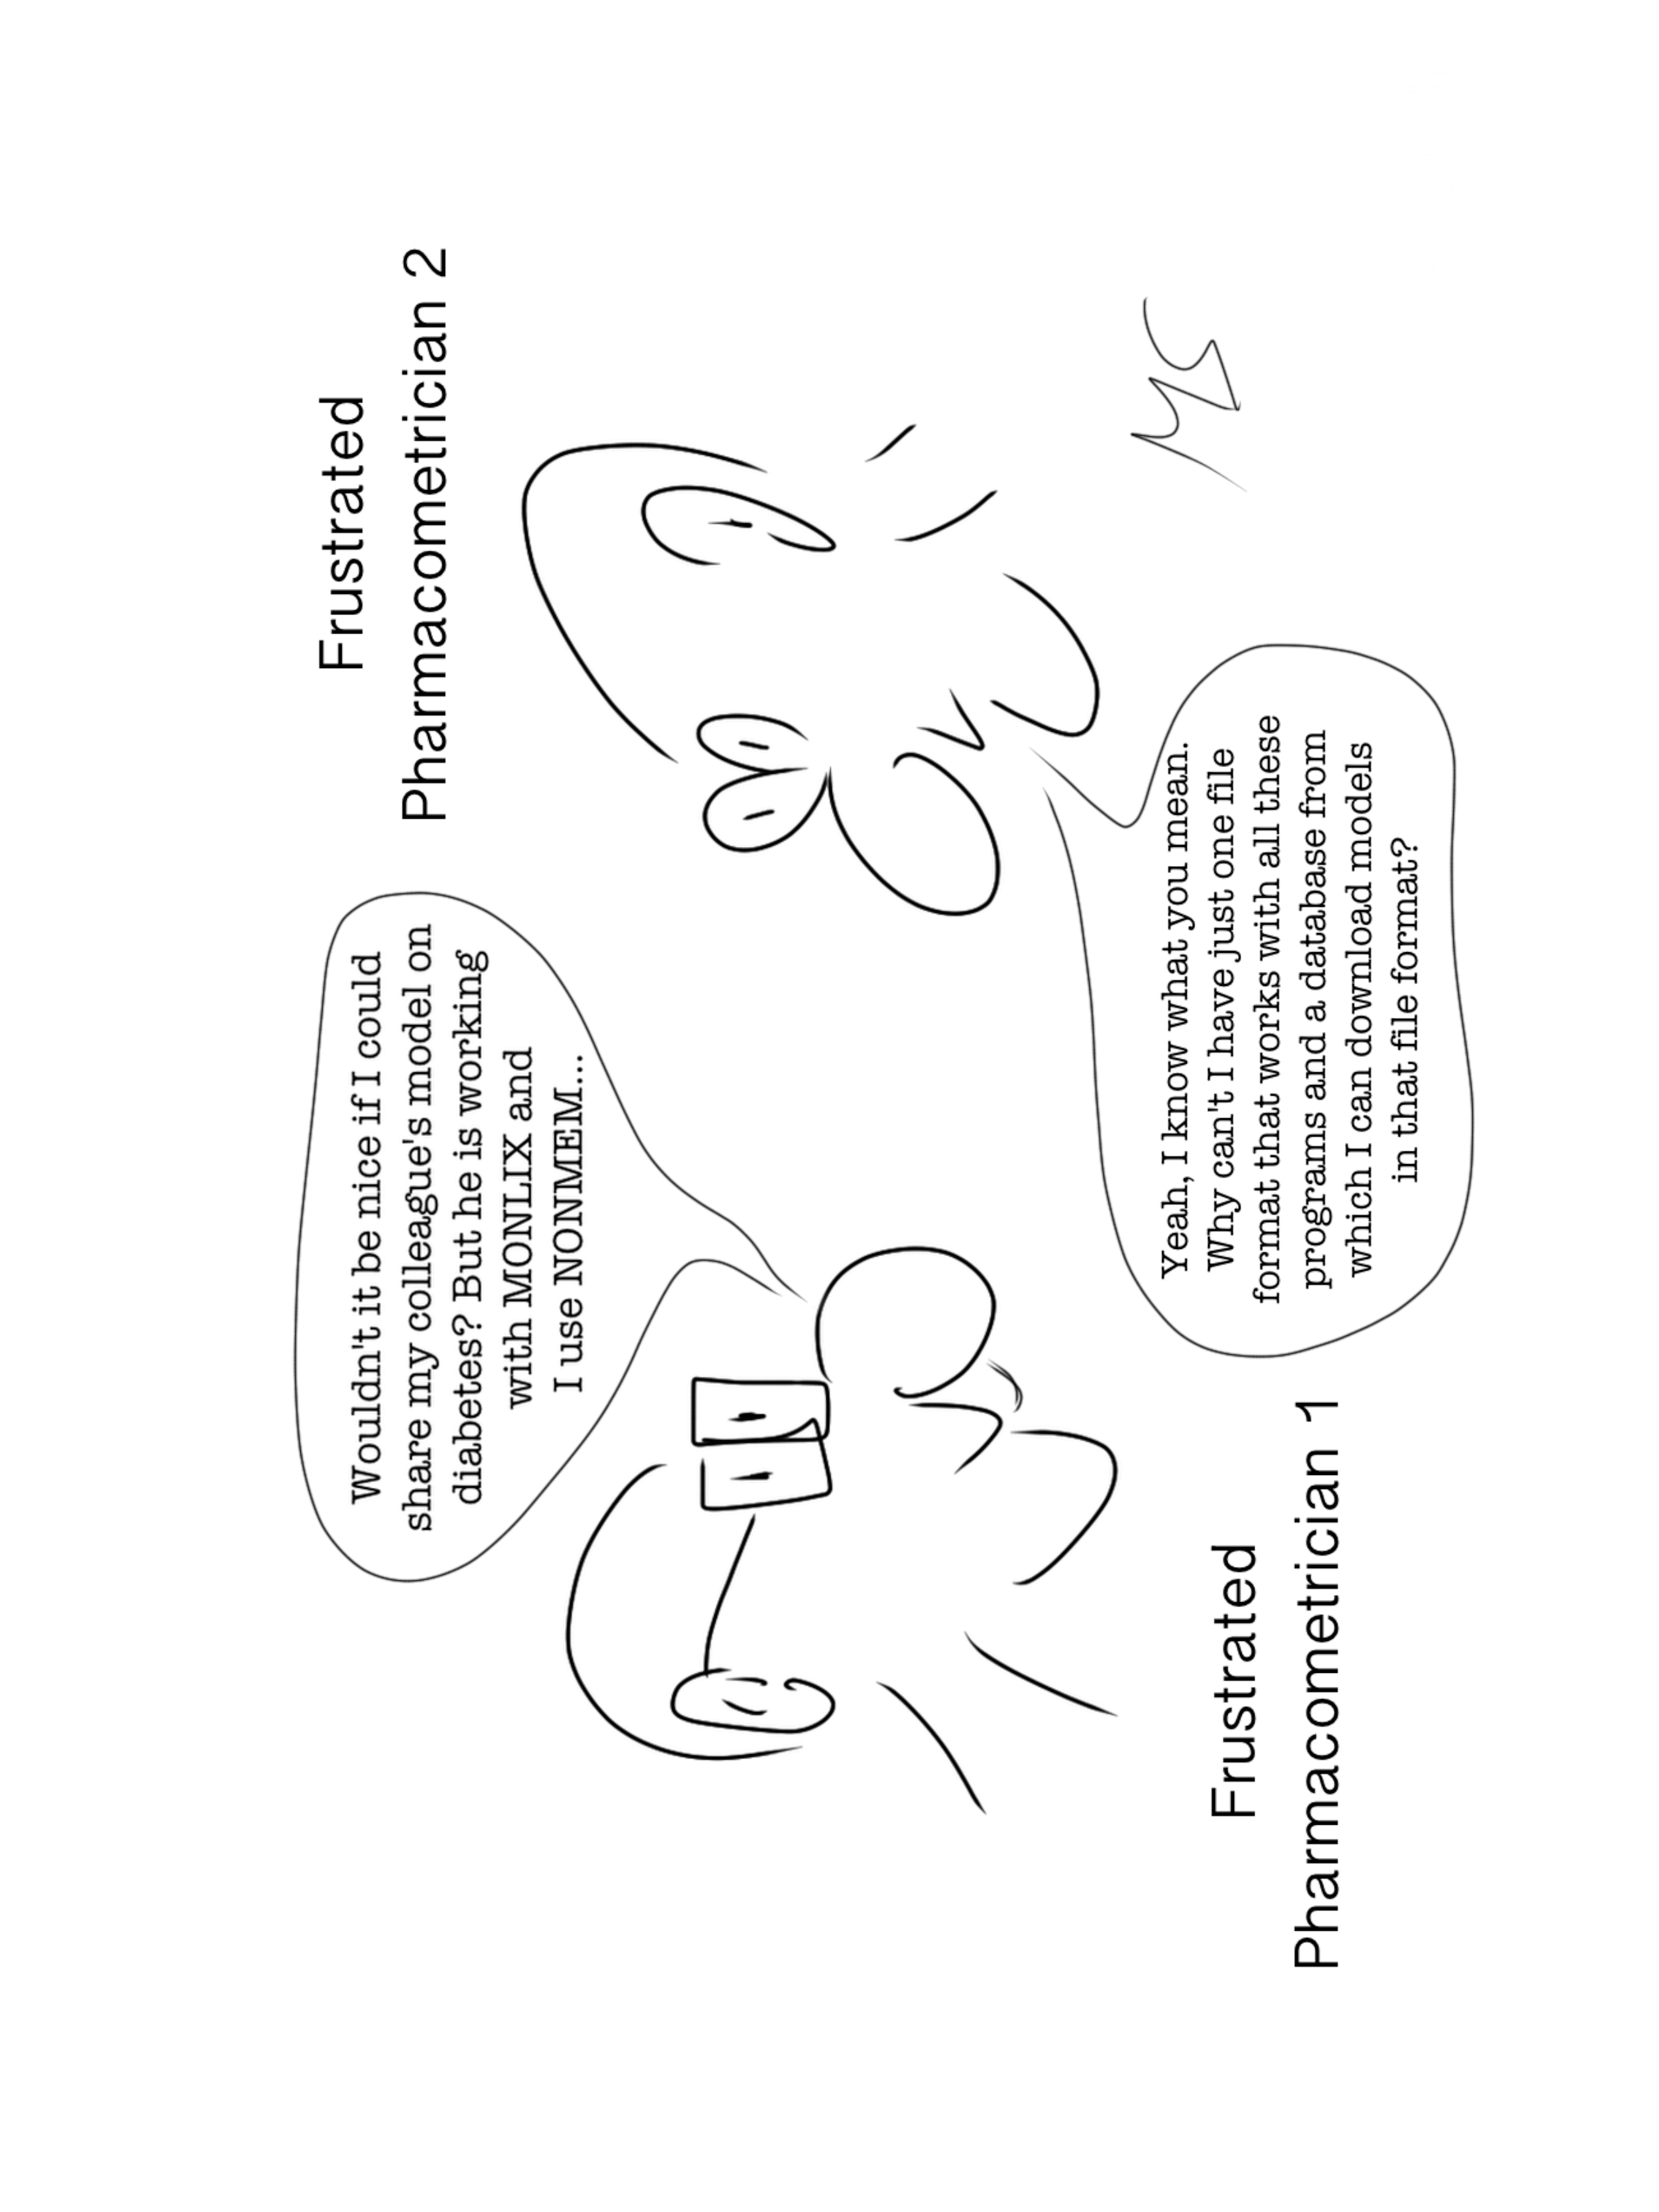
\includegraphics[angle=270,width=\linewidth,trim=90mm 80mm 80mm 50mm]{MMLdudesFinal2}
\end{wrapfigure}
% }
%\end{figure}

%We could add to this cartoon, the caption: ``Someone, somewhere must be trying to solve this problem!''
%And if you read the \ddmore newsletter\footnote{Available from \url{www.ddmore.eu}.}, where this cartoon first featured, you will recall that our reply was, ``Well fortunately they are!'' We think this

The cartoon on the right summarises the principal problem that \pharmml addresses: namely,
the reliable exchange of pharmacometric models between software tools. What we are aiming
for is illustrated in figure~\ref{fig:platformDDMoRe}, where \pharmml is the exchange medium
for pharmacometric models for the main modelling and simulation tools in the field. This is
not an unreasonable goal and has been successfully realised in the field of Systems Biology.

In Systems Biology the problems our Frustrated Pharmacometricans complain of do not exist. Software
tools exchange models using the Systems Biology Markup Language (SBML; \url{www.sbml.org})
\cite{SBML} and many published models can be found in the BioModels Database
(\url{http://www.ebi.ac.uk/biomodels-main/}) \cite{BioModels2010}. Modellers don't worry about the
content of an SBML file; they rely on the fact that when they exchange it between their favourite
modelling tools, it just works. Crucial to its success has been an active community of tool
developers and modellers who have supported and used it during
that time. Equally important has been the provision of sophisticated software libraries (libSBML
and JSBML) that take away much of the pain a software tool developer would otherwise experience
supporting what is now quite a complex standard. It is a virtuous circle. Users demand their
modelling tools support SBML\@. Developers provide reliable SBML support using libSBML, which
enables them to give their users what they want. The more tools that support SBML, the more useful
it becomes. The cost of supporting SBML is not negligible but quality libraries like libSBML make
the cost acceptable.

\begin{figure}[htb]
\centering
  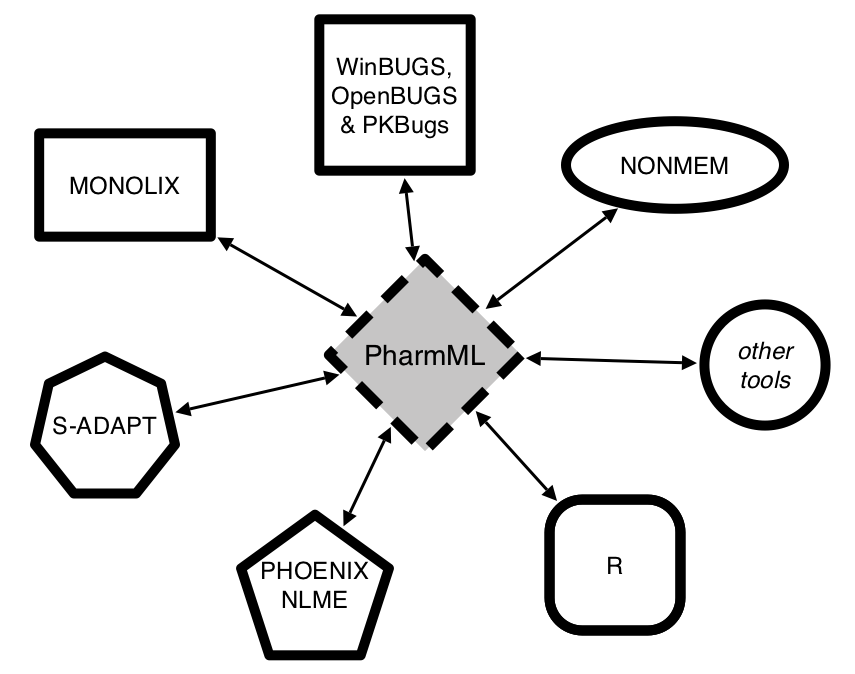
\includegraphics[width=0.5\linewidth]{platformDDMoRe}
 \caption{Interoperability platform to exchange models via \pharmml.}
 \label{fig:platformDDMoRe}
\end{figure}

This lesson has not be ignored by the pharmacometrics community and in fact a number of years
ago the NLME consortium (a consortium of pharmaceutical companies now all part of \ddmore) started
to work on a very similar standard to \pharmml. This resulted in early drafts of an XML based exchange
language, called PharML, but work on it was unfortunately discontinued and the standard has never been
used and validated. There are a number of other exchange standards in related modelling fields, which we
have drawn on in the development of our work to varying degrees, including:

\begin{description}
\item[CellML] Supports the exchange and storage of computer based mathematical models of biological systems \cite{CELLML}.
\item[NeuroML] Supports the exchange and description of models ``to describe the biophysics, anatomy and network architecture of neuronal systems at multiple scales''\footnote{Quoted from \url{http://www.neuroml.org} on 15 Mar 2013.} \cite{NeuroML}.
\item[NineML] Describes neuronal networks in a ``simulator independent language''\footnote{Quoted from \url{http://software.incf.org/software/nineml} on 15 Mar 2013.} that is design to interact with NeuroML \cite{ninemlspec}.
\item[SED-ML] Encodes simulation experiments of SBML and CellML models ``to ensure exchangeability and reproducibility of simulation experiments''\footnote{Quoted from \url{http://sed-ml.org} on 15 Mar 2013.} \cite{sedmll1v1}.
\end{description}

So what is the solution to the problem? \pharmml. An XML based language that will be able to encode
models from NONMEM, MONOLIX, BUGS and related tools. We intend this to be a community standard nucleated
around the members of the \ddmore consortium. In addition we are developing a software library
(libPharmML) to help tool providers incorporate support of \pharmml and to facilitate its
general adoption in the field.

So there is hope for the Frustrated Pharmacometricians. \pharmml will solve the problem.

% \begin{quote}
% {\small
% Nothing is original. Steal from anywhere that resonates with inspiration or fuels your imagination. Select only things to steal from that speak directly to your soul. If you do this, your work (and theft) will be authentic. Authenticity is invaluable; originality is non-existent. And don't bother concealing your thievery -- celebrate it if you feel like it. In any case, always remember what Jean-Luc Godard said: "It's not where you take things from -- it's where you take them to." \\
% \textit{Jim Jarmusch}}
% \end{quote}
% PharmML standardises the formulation and annotation of models used in pharmacometrics. Once a model is encoded in this format, it can flexibly be used for various purposes such as
% \begin{itemize}
% \item
% modelling
% \item
% simulation (e.g. individual subjects or clinical trial simulations)
% \item
% estimation (e.g. population and individual parameters)
% \item
% exploration (e.g. parameter scan/sensitivity, optimal design)
% \end{itemize}
% There are many tools being used in pharmacometrics, such as BUGS (winBUGS \cite{Lunn:2002aa} and openBUGS \cite{Lunn:2009fk}), Monolix \cite{Monolix4.2.1UserGuide:2012}, NONMEM \cite{NONMEM:2009}, PKBugs \cite{PKBUGS:1999}, S-ADAPT \cite{SADAPT:2008}, SimBiology Toolbox \cite{SimBiologyToolbox:2012} or Phoenix NLME \cite{PhoenixNLME:2011} to name only the the most popular.

% However, the current specification has been developed with focus on two tools being used in clinical and pharmaceutical research, NONMEM and Monolix. The choice and the number of tools under consideration had multiple reasons. On one side, the project description dictated the choice and preferences, on the other side the time constraints allowed for proper analysis of only these two tools. Further specifications will consider broader class of tools and approaches, such as Bayesian methods.

% Nevertheless, the differences between these softwares, which manifest themselves mainly in the \textit{imperative} approach of NONMEM versus the \textit{declarative} approach of Monolix, created a chance to a cover broad spectrum of methods and ideas developed over decades. \\
% On the one hand FORTRAN-based NONMEM, despite having a specifically defined language (NM-TRAN \cite{NONMEM:2009}), offers almost
% unlimited flexibility to the user. It can be viewed as a general purpose computational platform and in fact it has been developed
% as such and can be compared to Matlab or Mathematica (REFs). On the other hand Monolix has been specifically developed for use in pharmacometrics. Although being very flexible, it is based on MLXTRAN, a constantly developing declarative language, defining very precisely the types of allowed models and algorithms.
% \\
% It is not the purpose of this document to conduct a detailed comparison between these two approaches but it is important to keep the characteristic differences in mind. One of the main objectives of the DDMoRe project and specifically work-package 4 (WP4) is the building a bridging technology for alternative approaches within one framework. PharmML, the XML based exchange standard which is now available in this first specification is the core element of this interoperability framework.

% \begin{figure}[htb]
% \centering
%   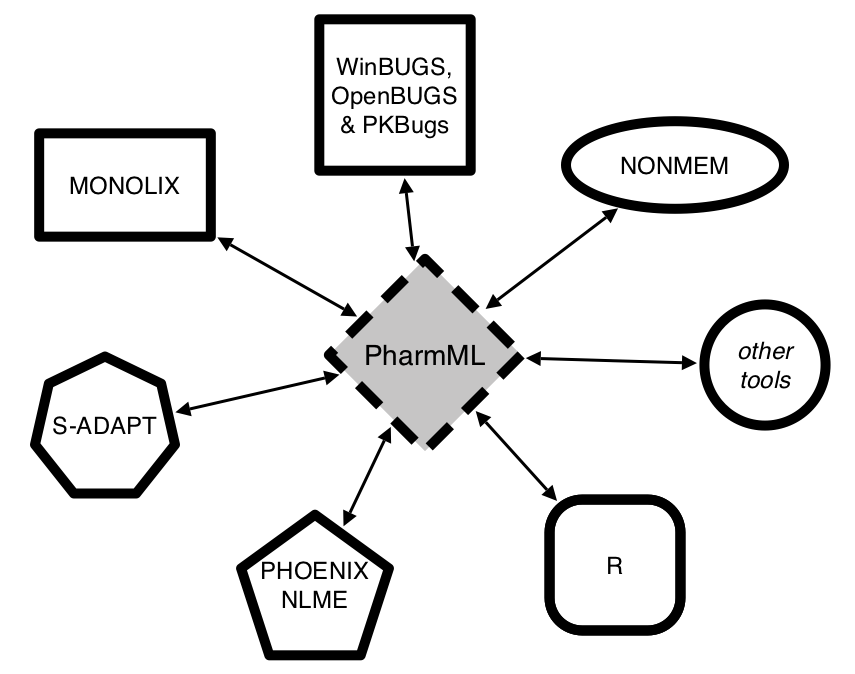
\includegraphics[width=0.9\linewidth]{platformDDMoRe}
%  \caption{Interoperability platform to exchange models via PharmML.}
%  \label{fig:platformDDMoRe}
% \end{figure}

% The idea of XML-based markup languages to represent models and data is not new. In fact, the pharmacometric community around the NLME consortium (REF) started to work on a new format for drug related research and developed an initial concept in form of the PharML standard (REF). The activities have been unfortunately discontinued and the standard has never been used and validated. There is number of other standards in various field of science, such as NeuroML (REF) in neurobiology, PMML (REF) in predictive analytics and data mining, SBML (REF) in Systems Biology or UncertML (REF) designed for encapsulating probabilistic uncertainties. PharmML builds on the experience and results of this effort by reusing those standards were appropriate.


% \section{Intro}

% I'm not sure about the quote at the beginning. I don't think it sets the correct tone. It also doesn't tie into the rest of the introduction. My preference would be to drop it or replace it with something that fits more neatly with what we are doing.

% I think this chapter could be expanded considerably and the current content reorganised.

% The current section doesn't mention the exchange of models, but says it can be used for M\&S, which is misleading. It makes it sound like a rival the MDL, which is it not. It goes on to state that the spec has focused on NONMEM \& Monolix, which is mis-leading as we have focussed on models generally (that why we had discussions with modellers and use general mathematical descriptions in the use case doc) but have wanted to ensure that we can support exchange between NONMEM and Monolix. I think this kind of statement would be better in the scope section. That way as the scope changes we don't need to update chap1 for future revisions. Then the discussion about the nature of imperative or declarative model specification languages, while useful comes far too soon (para 4). I think this should be a later section in this chapter, because it is important to mention it. The last paragraph about other MLs again should be expanded into a full section. It would be useful to go into some detail about SBML and libSBML. Also to include SED-ML too. Also perhaps the COMBINE archive - not sure about that one.

% The following is perhaps a better structure. I think breaking it into the following sections would be a good idea.


% \section{The Problem}

% We should set out the problem. That there is no platform independent way to exchange Pharmacometric models. We should also explain why this is desirable, i.e. what problems it would solve. Perhaps use the analogy of exchanging doscuments using word. No-one cares what the file looks like - it just works most of the time.

\section{The Solution}
\label{intro:objectives}

Having described the problem, we here articulate the \emph{kind} of solution we wanted \pharmml to be.
Developing a language as complex as \pharmml is a difficult undertaking and we wanted to make sure
that we had some firm principles in place to help when designing the language. We've set these aims
and objectives below. \pharmml should:

\begin{description}
%\item[encode models used by pharmacometricians]
\item[describe the mathematics of a model] The language should not include information about the authorship of a model, its update history, or the nature of the disease process or drug that is being modelled. These aspects will be captured by the annotation of the \pharmml document and are out of scope of this specification.
\item[describe the task(s) associated with a model] The task(s), such as simulation or estimation, to be performed with a model should be encoded in the language.
\item[be declarative] The language should describe \emph{what} information is present in a model and \emph{what} the associated task(s) are. It should not describe \emph{how} the information is organised, or \emph{how} the task(s) should be performed.
\item[be platform independent] Language elements specific to a particular modelling tool should not be included. For example it should not describe a structural model using a name specific to PREDPP in NONMEM.
\item[serve as an exchange format for the \ddmore infrastructure] The language should either support features required by the infrastructure or provide extension mechanisms so that additional information can be associated with the \pharmml document.
\item[provide support for ontological annotation] The language should provide a mechanism for it to be annotated with information that is useful to describe the model, but which is beyond the scope of the \pharmml document itself.
\item[enable custom extension] Provide an extensibility mechanism so that software tools can associate additional, possibly tool specific information, with a \pharmml document.
\item[reuse existing standards where appropriate] Where an established information standard exists that can be used to represent information within the \pharmml document, we should adopt it.
\end{description}

% Here we say what our aims and objectives were in designing PharmML. This is different to scope because it describes the high-level aims and objectives for PharmML that will not change in future releases of the standard. For example:

% - encode models used by pharmacometricians
% - platform independence
% - declarative
% - describe the mathematics of the model. For example, not the underlying medical condition or drug it is modelling (that is annotation/metadata).
% - Describe model and task
% - Serve as an exchange format for WP2 infrastructure.
% - Provide support for ontological annotation
% - Enable custom extension.
% - Reuse existing standards where appropriate.

\section{The \ddmore Consortium}

%Taken from the DDMoRe website need more work.

The Drug Disease Model Resources (DDMoRe) consortium aims to promote collaborative drug and disease
modelling and simulation research. Its aim is to develop tools and standards that will help the
consortium members and later the wider scientific community achieve this goal. Providing \pharmml
is a key goal of the consortium as it underpins a number of related deliverables of the consortium.
In particular:

\begin{itemize}
\item The \ddmore infrastructure in which \pharmml is used to exchange models between the different modelling tools.
\item The \ddmore model repository in which \pharmml will be used to upload and export models to and from the repository. It will also serve as the storage medium for the repository.
\item The \ddmore library of reference models and data-sets, which will provide models in several therapeutic areas. These models will be encoded using \pharmml.
\end{itemize}

The contribution of the \ddmore consortium members in guiding and reviewing the standard has been enormous.
As the standard evolves their role in using and then promoting the standard to the wider community will be invaluable.

\section{How \pharmml was developed}

We, the authors, have organised and designed \pharmml, but its development has very much been a
collaborative process. When embarking on this project we had a number of development guidelines that we adhered to.
We aimed to:

\begin{itemize}
\item start with a limited scope and expand the functionality we encode over time.
\item drive development using use cases which reflect the current scope.
\item test the implemented use cases by generating executable models.
\item have frequent review meetings with experts to make sure we are on the right track.
\item use existing technology standards if it is possible and reasonable to do so.
\item use existing information standards if applicable to avoid re-inventing the wheel.
\item make sure the standard is in a form and uses names and terms that make sense to the expert community.
\end{itemize}

The use-case based development cycle is illustrated in figure \ref{fig:devcycle} and you can see
how the generation of `executable' prototype models was important in ensuring assumptions were
correct before expanding the scope of the design. For this to be possible the use cases were
documented with a mathematical description and the expected outputs and results of the model were
also described in detail \cite{Swat:2013aa}. In some cases reference \matlab\xspace implementations were also included to
assist prototype code generation. Although this development cycle was our objective, in the later
stages there was insufficient time to upgrade the code generation framework to produce executable models
from a \pharmml document. Consequently some parts of the specification, in particular the parts related
to estimation tasks, have not been tested as thoroughly as we would like.

\begin{figure}[htb]
\centering%
 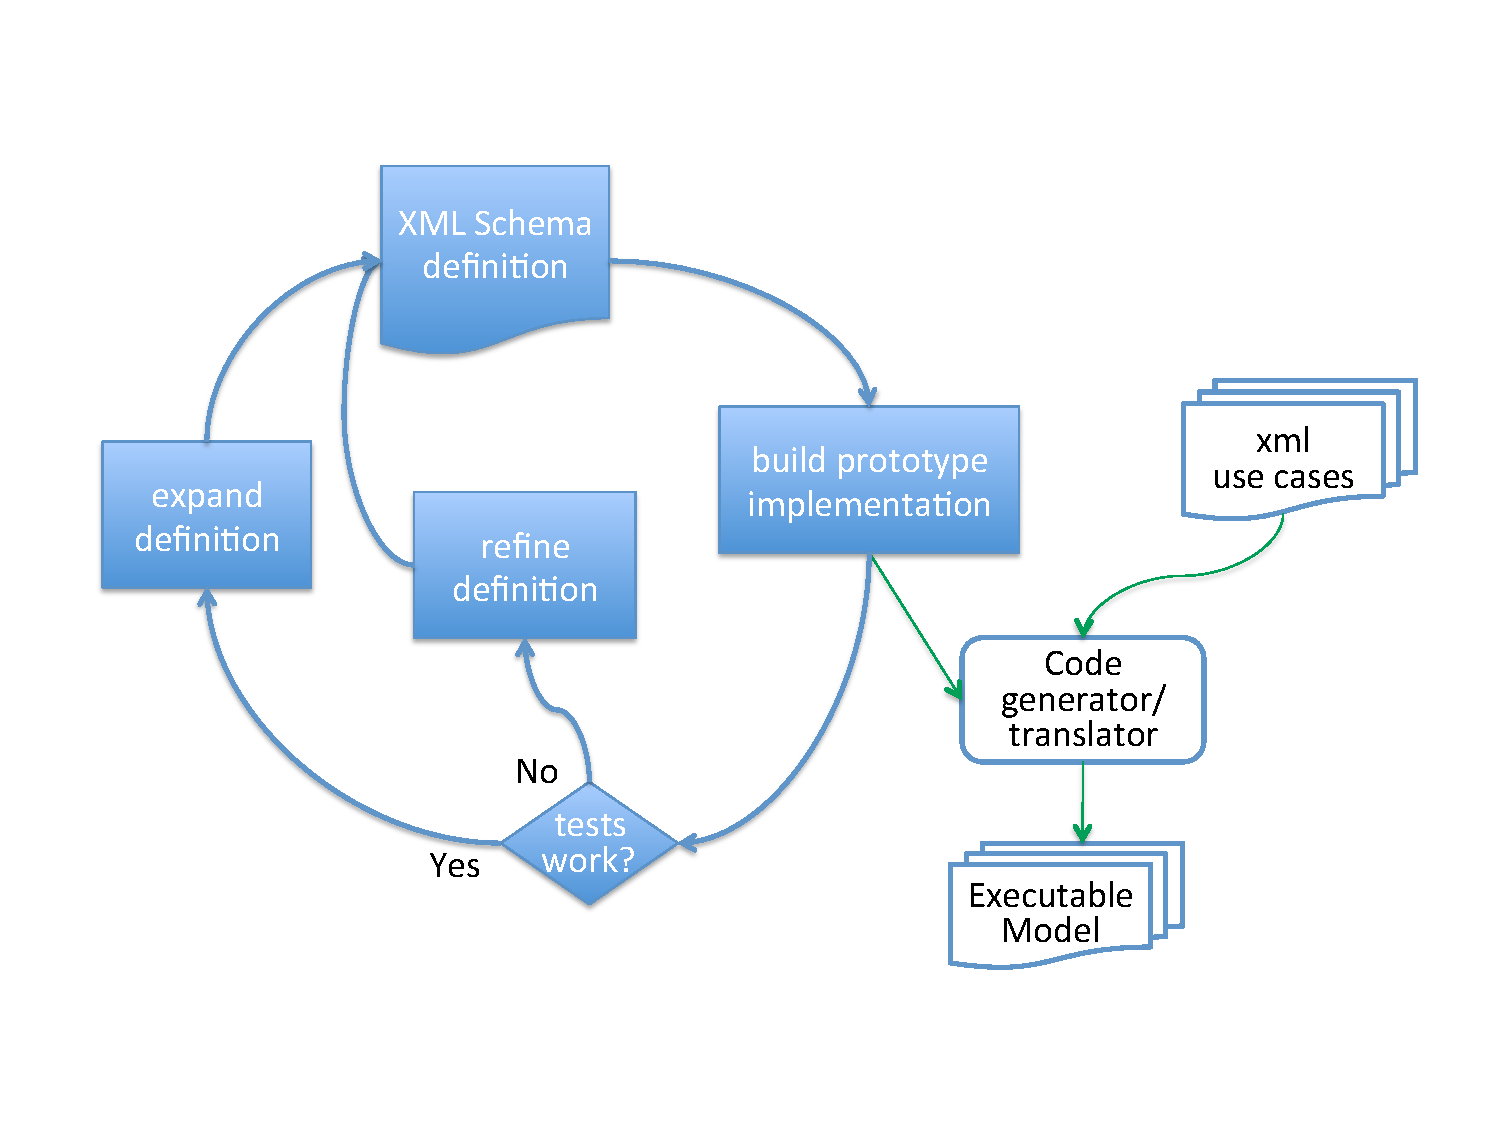
\includegraphics[width=0.7\linewidth,trim=10mm 20mm 20mm 10mm]{devcycle}
\caption{An overview of the development cycle adopted by the \pharmml team.}
\label{fig:devcycle}
\end{figure}


Peer review is important in the development of \pharmml and to date we have hosted three face-to-face
review meetings since the development of \pharmml commenced in August 2011. These meetings were:

\begin{itemize}
\item The \ddmore consortium meeting in Leiden, 24--26 Apr 2012.
\item The \ddmore consortium meeting in Noordwijkerhout, 11--13 Sep 2012.
\item The \ddmore technical workshop hosted by Novo Nordisk in Copenhagen, 28--30 Jan 2013.
\end{itemize}

\section{Imperative or Declarative?}

In developing \pharmml we have designed it to be a declarative language (see section \ref{intro:objectives}).
While we feel this is the best approach to take for an information exchange langage, it does present us
with number of challenges when dealing with NONMEM, the leading tool in the field. Despite
having a specifically defined language (NM-TRAN \cite{NONMEM:2009}), NONMEM offers a lot of flexibility
to the user, and experienced users can make NONMEM do things that it was never designed to do, to a large
extent because the imperative approach used in NONMEM facilitates this.

The challenge is to convert from the imperative to the declarative language, because there are usually many
ways to do the same thing in the imperative language. Therefore, generating a \pharmml document from a NONMEM
control stream may be challenging.

 % It is not the purpose of this document to conduct a detailed comparison between these two approaches but it is important to keep the characteristic differences in mind. One of the main objectives of the DDMoRe project and specifically work-package 4 (WP4) is the building a bridging technology for alternative approaches within one framework. PharmML, the XML based exchange standard which is now available in this first specification is the core element of this interoperability framework.

 % Nevertheless, the differences between these softwares, which manifest themselves mainly in the \emph{imperative} approach of NONMEM versus the \emph{declarative} approach of Monolix, created a chance to a cover broad spectrum of methods and ideas developed over decades. On the one hand FORTRAN-based NONMEM, despite having a specifically defined language (NM-TRAN \cite{NONMEM:2009}), offers almost
 % unlimited flexibility to the user. It can be viewed as a general purpose computational platform and in fact it has been developed
 % as such and can be compared to Matlab or Mathematica (REFs). On the other hand Monolix has been specifically developed for use in pharmacometrics. Although being very flexible, it is based on MLXTRAN, a constantly developing declarative language, defining very precisely the types of allowed models and algorithms.

 % It is not the purpose of this document to conduct a detailed comparison between these two approaches but it is important to keep the characteristic differences in mind. One of the main objectives of the DDMoRe project and specifically work-package 4 (WP4) is the building a bridging technology for alternative approaches within one framework. PharmML, the XML based exchange standard which is now available in this first specification is the core element of this interoperability framework.

%Let's put the NONMEM Monolix discussion here and then say that we have adopted a declaritive approach and say why it is better. Need to be careful %here to make sure we don't imply that in consequence Monolix is better than NONMEM.

\section{The Evolution of PharmML}

This document represents the start of an evolution for \pharmml. Any piece of software is upgraded as
users request new features and developers find better ways to do the same thing. A successful standard
is no different and with success in mind we expect \pharmml to evolve and change as it is subject to the
same influences. To manage this process we plan to adopt the following strategy to record versions of
the \pharmml specification.

\subsection{Version number}
\label{intro:versioning}

To record changes in the specification we will use the following three level numbering system, of the form
$x.y.z$. The levels correspond to the following types of revision:

\begin{description}
\item[$x$ major] Significant new features or radical change of design. Not backwards compatible.
\item[$y$ minor] New features or evolutionary design changes. Always backwards compatible.
\item[$z$ patch] Error corrections. Always backwards compatible.
\end{description}

By backwards compatible we mean that a \pharmml parser that supports version 1.9.0 must be able to read
a file that is compliant with version 1.4.0 of the \pharmml specification.

\subsection{Release Process}

Before each release we will submit a release candidate of the specification to the community for comments
and criticism. This is typically called a Request for Comments (RFC) and is standard practise. Based on
review comments the specification will either be revised, possibly significantly, and submitted for review
again or (if revisions are minor) revised and released.

The RFC period for this specification will end on 26 April 2013.

\section{Feedback}

Whether it is during the RFC process or after a release your feedback is important to us. Typically,
this feedback will be in the form of a specific issue: either to report defects you have identified in
the specification or to request new features. Either way we would urge you to submit specific issues to
our tracker at: \url{sf.net/ddmore/tracker}. In some cases you may wish to ask for clarification or raise
an issue that is broader than a specific issue or requires some discussion within the community. Here you
should contact the \pharmml forum at \url{sf.net/ddmore/forum}.
